%\todo{Algorithms and Techniques}
%\todo{- Explain PCA indetail }
%\todo{- Explain CNN in detail}
%\todo{Benchmark - define the benchmark and thresholds - this is already done}

\section{Principal Component Analysis}
TCE attributes set contains well over 200 attributes. I use the Principal Component Analysis to reduce the dimention of this dataset. Principal Component Analysis (PCA) is a standard method use in modern data analysis. PCA provides a roadmap for how to reduce complex data set to a lower dimension to reveal the something hidden, and simplified structures that often underline it. PCA reduces the dimensionality of the data set while preserving most of the variation in data. This talk is accomplished by identifying directions, called Principal Components, along which the variation in the data is maximal. Using this method, a dataset that has a large number of variables can be express using fewer variables (components). 

\subsection{Naive Basis}
 The goal of PCA is to identify the most meaningful basis to re-express the data set while filtering out the noise and expose hidden structures. Lets assume we have a dataset with $m$ number of variables. We can represent these data set using a $m$ orthogonal basises. without loss of generality, we can visualize a data set with a 3 variables using $x, y, z$ axises. $x,y,z$ axises are being the vatiables (Figure \ref{plot:3d}). In other words, the basis of this dataset is {(1, 0, 0), (0, 1, 0), (0, 0, 1)}. We can raise the question why we need to pick this basis over any other basis? The reason is that the naive basis reflects the method we gathered data. We can express this naive basis using matrix as follows 


\begin{figure}[!h]
\begin{center}
        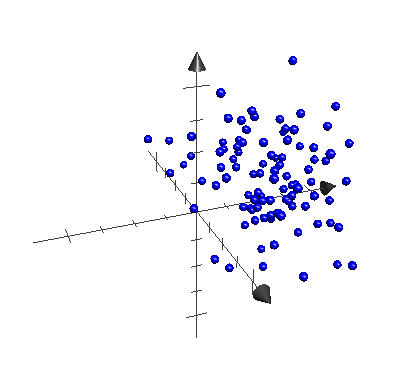
\includegraphics[width=0.4\textheight]{img/3D.png}
        \caption{Ax}  \label{plot:3d}
\end{center}
\end{figure}

\begin{equation}
%
    B =
	\begin{bmatrix}
    		b_{1}  \\
		b_{2}  \\
    		. \\
		b_{m}  \\
	\end{bmatrix}
	=
	\begin{bmatrix}
    		1 & 0 & 0 & \dots  & 0 \\
   		 0 & 1 & 0 & \dots  & 0 \\
    		\vdots & \vdots & \vdots & \ddots & \vdots \\
    		0 & 0 & 0 & \dots  &1
	\end{bmatrix}
	= I
%
\label{eq:I}
\end{equation}

Each row of this matrix is an orthonormal basis vector $b_{i}$ with $m$ components. All of our data has been recorded on this basis, and it can be expressed as a linear combination of ${b_{i}}$. Generalize form of the matrix can be written as a $m\times m$ identity matrix (Equation \ref{eq:I}).

\subsection{Change of Basis}

All the data has been recorded using naive basis; however, using linear algebra, we can find many other bases where these data can be re-express. For example, any rotation of naive basis will be perfectly valid basis to re-express the data. This is the question PCA precisely asking: Is there another basis, which is a linear combination of the original basis, which best re-express the data set?

Let us assume $X$ is our original data set and $Y$ is a new representation of the same data set.  We can perform a linear transformation ($P$) to produce $Y$ from $X$,

\begin{equation}
PX = Y
\label{eq:p}
\end{equation}

In matrix form, $P$ is a matrix that transforms $X$ into $Y$. Geometrically speaking $P$ rotate and stretch $X$ to produce $Y$. The rows of $P$ are a set of new basis vectors for expressing the columns of $X$.

\begin{equation}
%
    PX =
	\begin{bmatrix}
    		p_{1}  \\
		\vdots \\
		p_{m}  \\
	\end{bmatrix}
	\begin{bmatrix}
    		x_{1} & x_{2} & \dots  & x_{n} \\
	\end{bmatrix}
%
\label{eq:px}
\end{equation}

\begin{equation}
%
    Y =
	\begin{bmatrix}
    		p_{1}.x_{1} & \dots & p_{1}.x_{n} \\
		\vdots & \ddots & \vdots \\
		p_{m}.x_{1} & \dots & p_{m}.x_{n} \\
	\end{bmatrix}
%
\label{eq:y}
\end{equation}

Each column of $Y$ is a dot product of $x_i$ with the corresponding in $P$. Therefore, the rows of $P$ are a new set of basis vectors for representing of columns of $X$. 
It is important to mention that we are assuming the linearity and this reduce the problem to finding the appropriate change of basis. During this process, the row vector in the matrix P will become principal components. Now the question is what the criteria to pick the best possible basis P? The answer to this question is base on what features we would like Y to exhibit. 

Regardless the method of data analysis, the noise in the data must me low. If the noise in the data is significant, then the signal can not accurately extract.  The signal to noise ratio ($SNR$, Equation \ref{eq:snr}) or the proportion of variance sigma is high ($SNR >> 1$) for high precision data and low for noisy data.  best possible rotation for the naive basis is to find the basis that maximizes the $SNR$. This by assuming the dynamics of interest exists along directions with the largest variance. Therefore maximizing the $SNR$ allow us to find the best possible principal components. Finally, we can assume the Principal Components are orthogonal; this assumption provides an intuitive simplification that makes PCA solvable by using linear algebra decomposition techniques. 
\begin{equation}
SNR = \frac{\sigma^{2}_{signal}}{\sigma^{2}_{noise}}
\label{eq:snr}
\end{equation}

\subsection{Solving PCA using Eigenvalue Decomposistion}


One of the ways to find the PCA is using eigenvalue decomposition techniques. The first step is to find some orthonormal matrix $P$ (Eq \ref{eq:p}) by satisfying 
\begin{equation}
C_Y = \frac{1}{n} YY^{T}
\label{eq:cy}
\end{equation}


 $C_Y$is a diagonal matrix. The rows of $P$ are the principal components of $X$. Using simple substitutions using equation \ref{eq:p} and \ref{eq:cy}, we can derive $C_Y$ as, 

\begin{equation}
C_Y = P(\frac{1}{n}XX^{T})P^{T}
\label{eq:cy1}
\end{equation}

$\frac{1}{n}XX^{T} = C_X$ is the covariance matrix of X. Covariance matrix is a square matrix that has the variance of particular measurement types in diagonal terms, and off-diagonal terms are wth covariance between measurement types.  $C_X$capture the covariance between all possible pairs of measurements. Covariance values reflect the noise and redundancy in the measurements. In the diagonal terms, by assumptions, large values correspond to interesting structure, and in the off-diagonal terms, large values correspond to high redundancy. 

During the AVD, choice of $P$ diagonalizes $C_Y$. This was the goal of PCA. The results of the PCA can summarize as, 
\begin{itemize}
  \item The principal components of $X$ are the eigenvectors of $C_X$
  \item The ith components of $C_Y$ is the variance of $X$ along $p_i$
\end{itemize}


In practice computing PCA of a data set X is:

\begin{itemize}
  \item  Subtract off the measurement types
  \item  Computing the eigenvectors $C_X$
\end{itemize}


\section{Application of Artificial Neural Networks in Astrophysics}
In recent years, artificial neural networks (ANNs) have emerged as one of the potentially most successful modeling approaches in engineering and science. In this project, I am using backpropagation multilayered perceptron artificial neural network classifier to classify TCE catalog to identify planetary candidates. By using ANN, my objective is to apply machine learning technique to astrophysical datasets. 

ANNs are model after human brain and nervous system to simulate complex networks using interconnected modules. ANNs learn by examples; we call this a training data in which an actual measured set of input variables and the corresponding outputs are represented to determine the rules that govern the relationship between the variables. ANNs are well suited to modeling complex problems where the relationship among variables are not apparent and non-linear \cite{maier1995use}. The concept of artificial neurons was first introduced in 1943 \cite{mcculloch1943logical}, and since the back-propagation training algorithm for feed-forward was published in 1986 \cite{Rumelhart:1986:LIR:104279.104293}, ANNs has taken a significant advancement within last decade thus be considered as relatively new tool in the field of machine learning.

\subsection{Artificial Neural Networks}
ANN consists of a number of artificial neurons (also known as processing elements, nodes, or units). These neurons are usually arranged in layers. There are three different layers we can identify in ANN: an input layer, output layer and more layers between input and output collectively call hidden layers (Figure \ref{fig:ann}). 

\begin{figure}[!h]
\begin{center}
        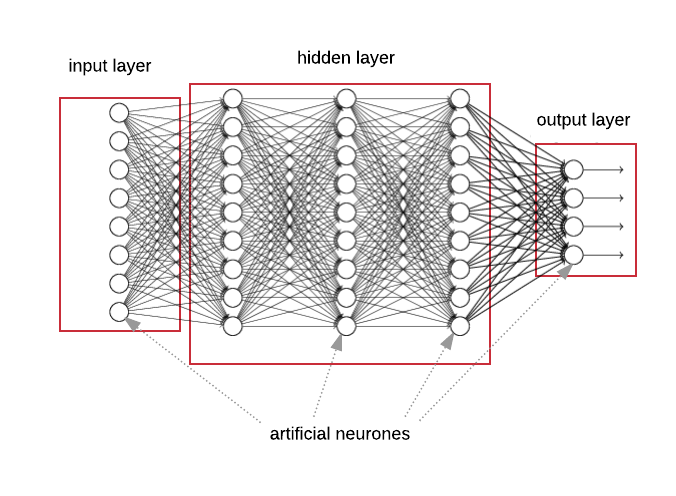
\includegraphics[width=0.7\textheight]{img/ann.png}
        \caption{Typical Structure of ANNs}  \label{fig:ann}
\end{center}
\end{figure}


\begin{figure}[!h]
\begin{center}
        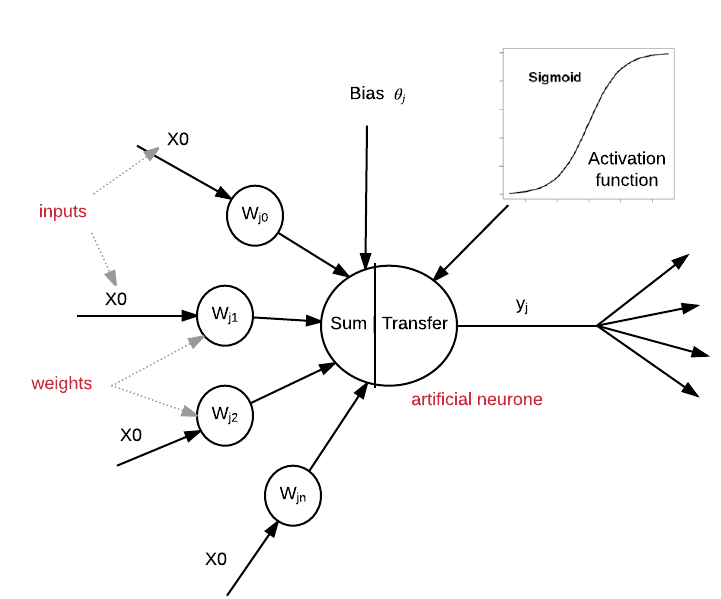
\includegraphics[width=0.6\textheight]{img/an.png}
        \caption{Artificial Neuron}  \label{fig:an}
\end{center}
\end{figure}

Each neuron is a layer partially or entirely connected to many other neurons via weighted connections. The scalar weights determine the strength of the connections between interconnected neurons. A zero weight means no connection between neurons and a negative weight refers to a prohibitive relationship. As shown in the Figure \ref{fig:an}, a neuron receives its weights inputs from other neurons which are summed, and a bias unit or threshold is added to subtracted. Bias us used to scale the input to a useful range to improve the convergence properties of the network (Equation \ref{eq:sum}).

\begin{equation}
I_j = \theta_j + \sum_{i=1}^{n} w_{ji}x_i
\label{eq:sum}
\end{equation}

Summed inputs $I_j$ pass through a transfer function to produce the output of the neuron. Figure \ref{fig:an} show this process for a neuron $j$ (Equation \ref{eq:transfer}).

\begin{equation}
y_j = f(I_J)
\label{eq:transfer}
\end{equation}

Using a predefined data set, that has known outputs for given inputs, and the network can be trained. The training steps are follows.

\begin{itemize}
\item Information propagation starts from the input layer where the data being fed to the network.
\item Inputs are weighted and received by each node in the next layer. 
\item Weighted inputs are summed and pass through a transfer function to produce neuron outputs, and pass to the neuron in the next layer. 
\item This process will be repeated while adjusting the weights to produce the predefined output of the training dataset. These weights are calculated by reducing the error.  
\end{itemize}


Learning in ANNs is usually divide into two separate groups: supervised and unsupervised \cite{mcculloch1943logical}.  Supervised learning neural network is given with a dataset with knows classifications (outputs), this dataset is known as the training data. During this project, I am using the supervised learning method to train the network. In this case, the network has been presented with TCE dataset with known planetary classifications. Network compare the known classification with the network output and compute the error. This error is used to adjust the weights among the neurons until the network produces the same results as the knows classifications in the training dataset. Two examples of Supervised learning ANNs are Multi-Layer Perceptrons (MLP) and neurofussy networks. In unsupervised learning, the network is only presented with the inputs without any desired outputs. The system itself adjusts the connection weights and cluster the input data records into classes of similar features.  ANNs also can be divided into two separate groups based on connection types among neurons: feedback networks and connections are in both forward and backward directions. During this project, I am using MLPs trained with a back-propagation algorithm. This has a high capacity of data mapping capabilities. 

\subsection{Multi-layer Perceptrons}
\label{sec:mlp}
In multi-layer perceptrons (MLPs) are fall under supervised feed-forward category in which the processing elements are arranged in a multilayered structure \cite{Introduction_to_the_theory_of_neural_computation} Figure \ref{fig:ann}.  As described in the equation \ref{eq:sum} and \ref{eq:transfer}, the input to a neuron is weighted and biased and run through an activation function before it passes on to the next layer. The output of a one neuron layer provides the input to the other next layer. The global error between the input and the output of the network is calculated using an error function. For example, the error function, for node j, is calculated using the equation \ref{eq:error}.

\begin{equation}
E = \frac{1}{2}\sum{(y_j - d_j)}^{2}
\label{eq:error}
\end{equation} 

where, $E$ is the global error function, $y_j$ is the predicted output by the network and $d_j$ is the desired output (from the training data set).

The objective is to minimize this error $E$ between the predicted and actual outputs. By reducing this error, the network can produce more accurate results. The minimization of this error function achieves with respect to all variables in the neural network such as connection weights, architecture, learning rate and threshold. Among these variables, connections weights are the most influential variable; thus back-propagation training algorithms are minimized the error function with respect to the connection weights only. Back-Propagation uses the gradient descent technique to adjust the weights in which the global error function, $E$ is minimized by modifying the weights using the equation \ref{eq:gd}.

\begin{equation}
\Delta{w_{ji}} = -\eta \frac{\partial E}{\partial w_{ji}}
\label{eq:gd}
\end{equation} 

where $\Delta{w_{ji}}$ is the weight increment from node $i$ to node $j$ and $\eta$ is the learning rate: the size of the step taken along the error surface is determined. 

The weights are then updated by adding the delta weight, xx to the corresponding previous weight as equation \ref{eq:weightupdate}

\begin{equation}
\Delta{w_{ji}}(n+1) = \Delta{w_{ji}}(n) + \Delta{w_{ji}}(n+1)
\label{eq:weightupdate}
\end{equation} 

where, $w_{ji}(n)$ is the value of the weight from node $i$ to node $j$ at step $n$ before the adjustment and $w_{ji}(n+1)$ is the value of the weight at step ($n+1$) after adjustment. 

\begin{equation}
\Delta{w_{ji}} = -\eta \frac{\partial E}{\partial w_{ji}} + \mu \Delta{w_{ji}}
\label{eq:momemtum}
\end{equation} 


First, the weights between the hidden and the output layers are adjusted, and then weights between the hidden layer and the input layers are adjusted. Learning rate is an another parameter we need to adjust in this process. Usually, the learning rate is adjusted by trial and error method. Smaller learning rate slows down the convergence even though the convergence can be achieved; however, it is subject to the local minima in the error surface that is closest to the random starting position. On the other hand, if the learning rate is large, the weight changes will be also large, causing the error to go up rather than down the thus convergence might never occur. However, larger learning rated might enable the model to jump out of local minima. Trial and error method to figure out the correct learning rate might lead us to oscillations, which can be overcome by adding another variable to the equation known as the momentum term ($\mu$). The process is to add a momentum term to the weight adjustment that is proportional to the amount of the previous weight change, Equation \ref{eq:momemtum}. Once the adjustments are carried out, it is saved and used to modify all the subsequent weight adjustments. This means that the weight change of the current step should carry some momentum of the weight change from the previous step. 

The process of adjusting weights is repeated until the network produce the desired results by minimizing the global error. Desired results are the output that given by the training data set. Once this process successfully calculates the proper weights, network continually can use these weights to make predictions, and at this point, we call this is a trained network that is ready to use in production. 

\begin{figure}[!h]
\begin{center}
        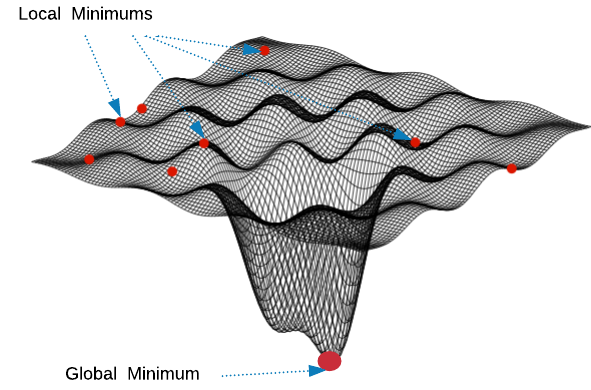
\includegraphics[width=0.4\textheight]{img/globalmin.png}
        \caption{Simulated error surface with local and global minimums. (Image credit: \url{https://projects.g-node.org/emoo/)}}  \label{fig:globalmin}
\end{center}
\end{figure}


Multi-layered perceptrons with back propagation algorithms are very efficient in many engineering problems; however, there are some limitations of this kind of neural networks. One of the limitation is that MLPs can get trapped in a local minimum in the process of finding the global minimum of the error surface. Exaggerated illustration of this issue is shown in figure \ref{fig:globalmin}. Gradient descent is working on reducing the error and trying to find the lowest error possible. As it shown in the figure  \ref{fig:globalmin}, there can be many local minimums presents in the error surface where the gradient descent may get trapped in local minimum even though there is a much apparent global minimum present.  In the literature, there are several ways proposed to escape from this local minima, including the learning rate, adding the momentum term, adding a small amount of random noise to the input patterns to shake the network from the line of steepest descent, adding more hidden nodes to relocating the network along the error surface by randomising the initial weights and retraining are some of them.Another limitation of MLPs is that feed-forward neural networks that are trained with the back-propagation are often criticized for being black boxes. The knowledge acquired by these networks during training is stored in their connection weights and bias values in a complex manner that is often difficult to interpret. 


To improve the performance of the ANN models,  we need to determine the model inputs carefully. Careful selection of the model inputs will significantly improve the performance of the network. Mostly we can choose the model input based on the prior knowledge of the problem we are aiming to solve. Another technique is to train many neural networks with different combinations of input variables and to select the network that has the best performance \cite{teh1997prediction}. There are many other techniques can be found in the literature to the best method to pick model inputs. Selecting a large number of input variables usually increase the network size resulting in a decrease in processing speed and reducing the efficiency of the network. 

Once the input parameters are selected, the dataset is divided into two separate sets: training and testing sets. Training set will be used to train and find out the connections weights and other network parameters by minimizing the error between model outputs and the corresponding measured values. Since ANN models have a large number of models parameters, this may cause to overfit the training data, especially if the training date are noisy. In other words, if the number of degrees of freedom of the model is huge compared to training date points, the model might no longer fit the general trend of the data. The testing data set used to make sure the model can generalize within the range of the data used for calibration. Usually, 2/3 of the data are recommended for a training dataset, and 1/3 will use as testing data.  If the available data are small, it is difficult to have enough data points in the training dataset hence the k-folding method can be used to separate dataset and train the network.  

Once the available data have been divided into training and testing, it is important to pre-process the data in a suitable form before they are applied to the ANN. Data pre-processing usually speed up the learning process. Pre-processing can be done in the form of data scaling (this allow the transfer function to perform well), normalization (in some cases the data need to be normally distributed to obtain optimal results) and transformation (transform the input data into some known form may be helpful to improve ANN performance). 


For free-forward neural networks, the most common method to find the optimum weight is the first order gradient descent. The advantage of this approach is that they have the ability to escape local minima in the error surface and thus produce optimal or near-optimal results. However, this also has a slow convergence rate. The stopping criteria are used to decide when to stop the training process. There are many criteria can be used to determine when to stop training: When the training error reaches a sufficiently small value. Or when not or slight changes in the training error occurred. However, the above example of stopping criteria may lead to the model ending permanently or over-training, and cross-validation approach can be used to overcome these problems. The cross-validation required to divide the data into three sets: training, testing and validating. 
 
\subsection{Model Validation}
The performance of the model validation ensures that the model has learned the complex and non-linear relations among variables using training data and is capable of generalized within limits. The standard approach is to achieve this is to test the performance of trained ANNs on the independent validation set, which has been using as part of the model building process. Prediction performance of ANN models are often evaluated using a couple of different methods: The coefficient of correlation (Equation \ref{eq:coefficient_of_correlation}) , root mean squared error (RMSE, Equation \ref{sq:rmse}) and mean absolute error (MAE, Equation \ref{sq:mae}).

\begin{equation}
r = \frac{C_{y_{j} d_{j}}}{\sigma{y_{j}\sigma_{d_{j}}}}
\label{eq:coefficient_of_correlation}
\end{equation}

where, $y_j$ - model (predicted) output, desired (observed) output, $C_{y_{j} d_{j}}$ covariance between the model output and desired output. Suggested values for $r$ are, 

\begin{itemize}
\item $|r| \ge 0.8$ - Strong correlation exists between two sets of variables. 
\item $0.2 < |r| < 0.8 $ - Correlation exists between eh two sets of variables 
\item $|r| \le 0.2$  - weak correlation exists between the two sets fo variables
\end{itemize}

RMSE is the most accepted measure of error and has the advantage that large errors receive much greater attention than small error.

\begin{equation}
RMSE = \sqrt{\frac{1}{n} \sum_{j=1}^{n}(y_j - d_j)^{2}}
\label{sq:rmse}
\end{equation}


\begin{equation}
MAE = \frac{1}{n} \sum_{j=1}^{n}|y_j - d_j|
\label{sq:mae}
\end{equation}

\subsection{Benchmark Model}

Benchmarking the neural network by performing many training trials by varying number of training data sets to reach the optimal network. Initial weight will be randomly chosen \cite{hamey1991benchmarking}. Comparing the performance of the NN with other classification algorithms also provide a degree of freedom to benchmark our model. In the literature there are many classification domains can be found that perform classification task on KOI dataset: K-nearest neighbors (K-NN) \cite{2011MNRAS.414.2602D}, Naive Bays \cite{feigelson2012}, Random Forests \cite{2015ApJ...806....6M}.

\begin{figure}[!h]
\begin{center}
        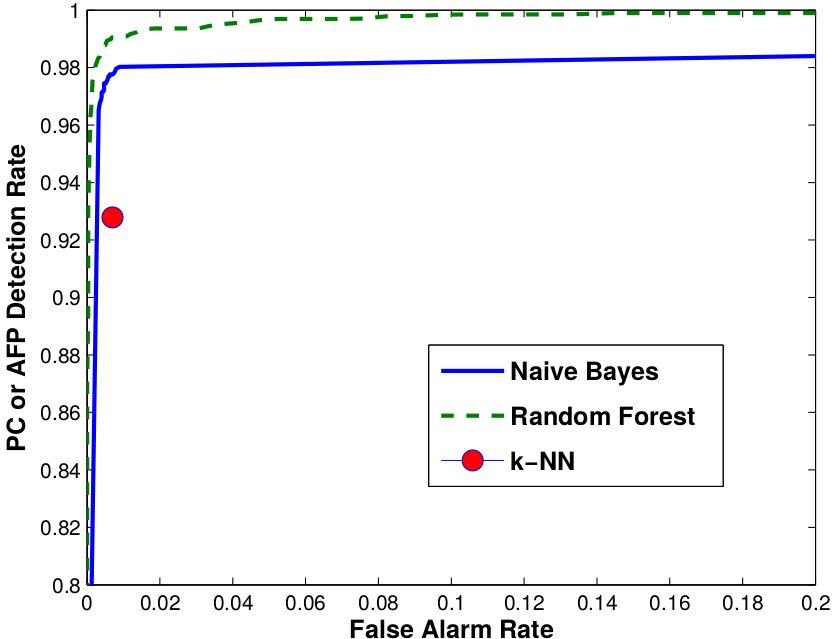
\includegraphics[width=0.35\textheight]{img/benchmark.png}
        \caption{Comparison of Random forest, Naive Bayes and K-NN. Image Credit: McCauliff et al. 2015 \cite{2015ApJ...806....6M}}  \label{fig:benchmark}
\end{center}
\end{figure}

Figure \ref{fig:benchmark} show PC or AFP Detection Rate vs False Alarm Rate of three different classification results performances. K-NN does not produce a ranking of predictions and so is represented as a single point in the plot. The resulting error rates for K-NN and Naive Bays are 3.15$\%$ and 2.73$\%$ respectively. I will be using these statistics that found in the literature as the benchmark for Neural Network using in this project.


